\documentclass{ctexart}

\usepackage{../jiajiao}

\graphicspath{{../figs/}}

\def\examplecolor{White}
\def\theoremcolor{White}
\def\remarkcolor{White}
\def\solutioncolor{White}

% 纸张大小,页边距
%\usepackage[a5paper,left=2.2cm,right=1.7cm,top=2.4cm,bottom=2.4cm]{geometry}
\usepackage[a4paper,left=3.8cm,right=3.2cm,top=3.4cm,bottom=3.4cm]{geometry}

\begin{document}

\section{2020 年 12 月 5 日答疑记录}

\subsection{函数的零点与方程的根}

  求方程的根可以转化为求对应函数图形交点的横坐标, 或求对应函数的零点. 
  一般有如下两种转化方法:
  \begin{align*}
    f(x)=0\text{\ 的根}&\Leftrightarrow 
      \text{$f(x)$ 的图形与 $x$ 轴交点的横坐标};\\
    f(x)+g(x)=0\text{\ 的根}&\Leftrightarrow 
      \text{$f(x)$ 与 $-g(x)$ 的图形交点的横坐标}.
  \end{align*}
  前一种方法可视为后一种方法的特例, 而两种方法在使用时都需要考虑函数的单调性.
  此外还有 (画图更容易理解)
  
  \myemph{零点存在性定理}: 若 $f(x)$ 在 $[a,b]$ 上连续, 且 $f(a)f(b)<0$, 
  则 $f(x)$ 在 $(a,b)$ 上至少有一根. 

\begin{example}\label{exa:201217-1900}
    已知函数 $f(x)= \begin{cases}
        \dfrac2x, & x\geqslant 2,\\
        x^2-3, & x<2,
    \end{cases}$ 若关于 $x$ 的方程 $f(x)=k$ 有三个不等的实根, 求 $k$ 的取值范围.
\end{example}
\begin{solution}
    此题应考虑函数 $y=f(x)$ 与 $y=k$ 的图形的交点恰有三个的情形. 画出两者的图形示意图, 容易知道 $k\in(0,1)$.
    
    \begin{center}
        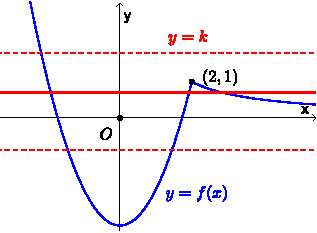
\includegraphics[scale=1]{2020-1214-1900-crop}
    \end{center}
\end{solution}

\begin{example}\label{exa:201214-1905}
    求函数 $f(x)=x^2-\log_{\frac12} x$ 的零点个数.
\end{example}
\begin{solution}
    由 $f(x)=x^2-\log_{\frac12} x=0$ 可得 $x^2=\log_{\frac12} x$, 故设 $g(x)=x^2$, $h(x)=\log_{\frac12} x$, 并考虑两者图形的交点个数. 画图可知, 只有一个交点.
    
    \begin{center}
        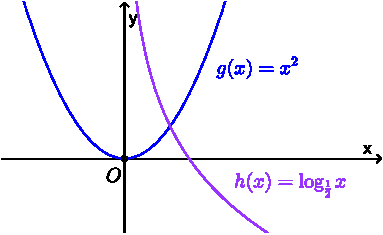
\includegraphics[scale=1]{2020-1214-1910-crop}
    \end{center}
\end{solution}
\begin{remark}
    可以进一步用零点存在性定理来估计例~\ref{exa:201214-1905} 中的 $f(x)$ 的零点所在的大致区间. 因为已经由图知道 $f(x)$ 的零点为正数, 所以只需考虑 $x\in(0,+\infty)$ 的情形. 又因为此时 $\log_{\frac12} x$ 单调递减, 而 $-\log_{\frac12} x$ 单调递增, 所以 $f(x)=x^2-\log_{\frac12} x$ 单调递增. 计算知, $f\biggl(\dfrac12\biggr)=-\dfrac34$, $f(1)=1$, 由零点存在性定理, 零点在区间 $\biggl(\dfrac12,1\biggl)$ 内.
\end{remark}

\begin{example}
    设函数 $f(x)= \begin{cases}
        x, & x<a,\\
        x^2, & x\geqslant a,
    \end{cases}$ 若对于任意实数 $b$, 关于 $x$ 的方程 $f(x)-b=0$ 总有实根, 求 $a$ 的取值范围.
\end{example}
\begin{solution}
    由 $f(x)$ 的表达式可知, 其图形在 $(-\infty,a)$ 上为直线 $y=x$ 的一部分, 在 $[a,+\infty)$ 上为抛物线 $y=x^2$ 的一部分. 而方程 $f(x)-b=0$ 等价于 $f(x)=b$, 则 $a$ 的取值应使得 $y=f(x)$ 与 $y=b$ 的图形总有交点. 画图可知, 仅当 $a\in[0,1]$ 时满足题意.
    
    \begin{center}
        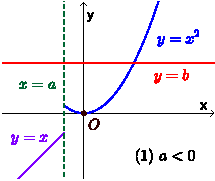
\includegraphics[scale=1]{2020-1214-1920-crop}\qquad
        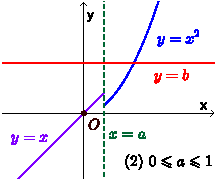
\includegraphics[scale=1]{2020-1214-1930-crop}\qquad
        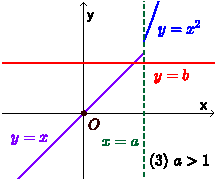
\includegraphics[scale=1]{2020-1214-1940-crop}
    \end{center}
\end{solution}

\begin{example}
    ``$t\geqslant 0$'' 是 ``函数 $f(x)= x^2+tx-t$ 在 $(-\infty,+\infty)$ 内存在零点'' 的什么条件? 
\end{example}
\begin{solution}
    函数 $f(x)= x^2+tx-t$ 在 $(-\infty,+\infty)$ 内存在零点的充要条件是 $\Delta= t^2-4(-t)\geqslant 0$ 即 $t\in(-\infty,-4]\cup [0,+\infty)$, 所以 ``$t\geqslant 0$'' 是 ``函数 $f(x)= x^2+tx-t$ 在 $(-\infty,+\infty)$ 内存在零点'' 的充分不必要条件.
\end{solution}

\subsection{解简单的指数、对数方程或不等式}

解简单的指数、对数方程或不等式, 一般是利用指数、对数的单调性 (参考 ``2020 年 11 月 21 日答疑记录''). 具体来说, 有两种方法.

方法一: 化为同底的指数或对数 (简记为 ``化同底''). 例如, 指数方程 $2^x=4$ 可化为 $2^x=2^2$, 由 $y=2^x$ 单调递增可知, $x=2$. 类似地, $\log_2 x= 2$ 可化为 $\log_2 x= \log_2 4$, 由 $y=\log_2 x$ 单调递增可知, $x=4$. 再如, $2^x>4$ 可化为 $2^x>2^2$, 则 $x>2$; $\log_{0.5} x> 2$ 可化为 $\log_{0.5} x> \log_{0.5} 0.5^2$, 由 $y=\log_{0.5} x$ 单调递减可知, $0<x< 0.25$. 注意, 对数函数有自然定义域, 即真数 (此处的 $x$) 大于零.

方法二: 直接取对数或构造指数式. 此方法涉及指数和对数的运算法则 (参考 ``2020 年 11 月 8 日答疑记录''). 例如, 对方程 $2^x=4$ 两边取以 $2$ 为底的对数, 可得 $\log_2 2^x= \log_2 4$, 即 $x=2$. 类似地, 将 $\log_2 x< 2$ 化为 $2^{\log_2 x}< 2^2$, 可知 $0<x<4$ (注意对数函数的自然定义域). 再如, 由 $2^x>3$ 可得 $x>\log_2 3$ (这个例子用前一个方法来解并不方便). 在这些例子中, 新构造的对数式或指数式的底均应与原式中的相同.

\begin{example}
    解下列不等式: 
    
    (1) $\biggl(\dfrac12\biggr)^x>4$;\qquad
    (2) $\log_3 x> 2$;\qquad
    (3) $3^{x^2+x}>9$;\qquad
    (4) $\log_5 (x^2-4x)\leqslant 1$.
\end{example}
\begin{solution}
    (1) 方法一: 不等式化为 $\biggl(\dfrac12\biggr)^x> \biggl(\dfrac12\biggr)^{-2}$, 所以 $x\in(-\infty,-2)$.
    
    方法二: 不等式化为 $\log_{\frac12}\biggl(\dfrac12\biggr)^x< \log_{\frac12} 4= \log_{\frac12} \biggl(\dfrac12\biggr)^{-2}$, 所以 $x\in(-\infty,-2)$.
    
    (2) 方法一: 不等式化为 $\log_3 x> \log_3 9$, 所以 $x\in(9,+\infty)$.
    
    方法二: 不等式化为 $3^{\log_3 x}> 3^2$, 所以 $x\in(9,+\infty)$.
    
    (3) 方法一: 不等式化为 
    \[3^{x^2+x}>3^2,\quad\text{即}\quad x^2+x>2,\]
    解得 $x\in(-\infty,-2)\cup (1,+\infty)$.
    
    方法二: 不等式化为 $\log_3 3^{x^2+x}>\log_3 9$, 仍可解得 $x\in(-\infty,-2)\cup (1,+\infty)$.
    
    (4) 方法一: 不等式化为 
    \[\log_5 (x^2-4x)\leqslant \log_5 5,\quad\text{即}\quad 0<x^2-4x\leqslant 5,\]
    解得 $x\in[-1,0)\cup (4,5]$.
    
    方法二: 不等式化为 $5^{\log_5 (x^2-4x)}\leqslant 5^1$, 仍可解得 $x\in[-1,0)\cup (4,5]$.
\end{solution}
\section{2020 年 12 月 6 日答疑记录}

\subsection{图形变换}

先考虑函数 $y=f(x)$ 与 $y=f(x+1)$ 的图形. 因为点~$A(n,f(n))$ 满足 $y=f(x)$ (此时 $x=n$), 而点~$A'(n-1,f(n))$ 满足 $y=f(x+1)$ (此时 $x=n-1$), 且点~$A$ 向左平移一个单位长度可得点~$A'$, 所以将 $y=f(x)$ 图形上的所有点向左平移一个单位长度可得 $y=f(x+1)$ 的图形.

再考虑函数 $y=f(x)$ 与 $y=f(x)+1$ 的图形. 因为点~$B(n,f(n))$ 满足 $y=f(x)$ (此时 $x=n$), 而点~$B'(n,f(n)+1)$ 满足 $y=f(x+1)$ (此时 $x=n$), 且点~$B$ 向上平移一个单位长度可得点~$B'$, 所以将 $y=f(x)$ 图形上的所有点向上平移一个单位长度可得 $y=f(x)+1$ 的图形.

设 $a>0$, 由同样的分析可以知道, 
\[\begin{aligned}
    &\text{向左平移 $a$ 个单位长度:}\ f(x)\rightarrow f(x+a);\\
    &\text{向右平移 $a$ 个单位长度:}\ f(x)\rightarrow f(x-a);\\
    &\text{向上平移 $a$ 个单位长度:}\ f(x)\rightarrow f(x)+a;\\
    &\text{向下平移 $a$ 个单位长度:}\ f(x)\rightarrow f(x)-a.
\end{aligned}\]
以上结论可以简记为 ``左加右减, 上加下减''. 示意图如下($a>0$):

    \begin{center}
        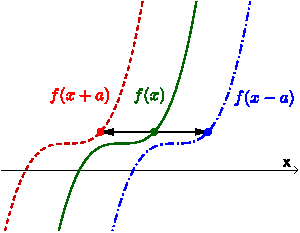
\includegraphics[scale=1]{2020-1215-1900-crop}\qquad
        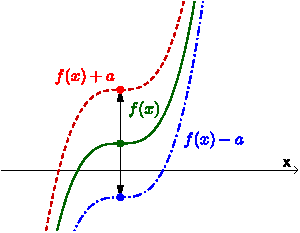
\includegraphics[scale=1]{2020-1215-1910-crop}
    \end{center}

注意, 这些结论均是对 $x$ 或 $f(x)$ (即 $y$) 的整体变换. 例如 $f(2x)$ 的图形往左平移 $1$~个单位长度, 得到 $f(2(x+1))$ 即 $f(2x+2)$ 的图形; 而由 $f(3x)$ 的图形要得到 $f(3x-1)$ 的图形, 需将前者往右平移 $\dfrac13$~个单位长度.

接着考虑函数 $y=f(x)$ 与 $y=-f(x)$ 的图形. 因为点~$C(n,f(n))$ 满足 $y=f(x)$ (此时 $x=n$), 而点~$C'(n,-f(n))$ 满足 $y=f(x+1)$ (此时 $x=n$), 且点~$C$ 与 $C'$ 关于 $x$~轴对称, 所以作 $y=f(x)$ 图形上的所有点关于 $x$~轴的对称点可得 $y=-f(x)$ 的图形 (两个图形上对应点横坐标相同, 纵坐标互为相反数, 简记为 ``上下翻转''). 类似地, 作 $y=f(x)$ 图形上的所有点关于 $y$~轴的对称点可得 $y=f(-x)$ 的图形 (两个图形上对应点横坐标互为相反数, 纵坐标相同, 简记为 ``左右翻转''). 示意图如下:

    \begin{center}
        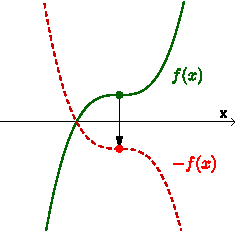
\includegraphics[scale=1]{2020-1215-1920-crop}\qquad
        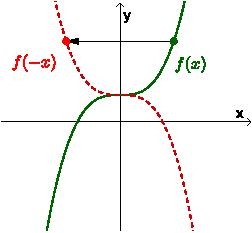
\includegraphics[scale=1]{2020-1215-1930-crop}
    \end{center}

上述六种图形变换可以叠加. 例如, $f(x)$ 的图形先上下翻转可得 $-f(x)$ 的图形, 再左右翻转可得 $-f(-x)$ 的图形; $f(x)$ 的图形先左右翻转可得 $f(-x)$ 的图形, 再向右平移 $4$ 个单位长度 (将 $x$ 替换为 $x-4$) 可得 $f(4-x)$ 的图形.

\begin{example}
    已知 $f(x)=\begin{cases}
        \dfrac12 x,& -2\leqslant x\leqslant 0,\\
        -x^2+2x,& 0<x\leqslant 2,
    \end{cases}$ 画出下列函数的图形:
    
    (1) $f(x)$;\qquad (2) $f(x-2)$;\qquad (3) $-f(x)$;\qquad 
    (4) $f(-x)$;\qquad (5) $-f(-x)$.
\end{example}
\begin{solution}
    各函数图形依次如下:
    
    \begin{center}
        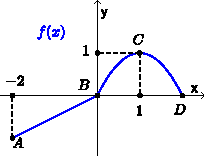
\includegraphics[scale=1.2]{2020-1215-1940-crop}\qquad
        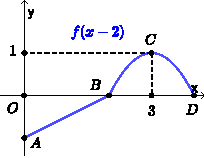
\includegraphics[scale=1.2]{2020-1215-1950-crop}\qquad
        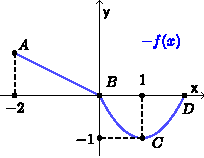
\includegraphics[scale=1.2]{2020-1215-2000-crop}
    \end{center}
    
    \begin{center}
        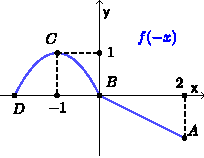
\includegraphics[scale=1.2]{2020-1215-2010-crop}\qquad
        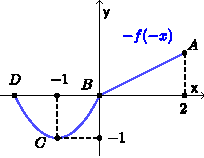
\includegraphics[scale=1.2]{2020-1215-2020-crop}
    \end{center}
\end{solution}

\subsection{恒成立问题}

恒成立问题一般化为值域问题来求解. 例如, 设 $D$ 为函数 $f(x)$ 的定义域, 则
\[\begin{gathered}
    \forall\, x\in D, f(x)\leqslant m\Leftrightarrow f_{\max}\leqslant m,\\
    \forall\, x\in D, f(x)\geqslant m\Leftrightarrow f_{\min}\geqslant m.
\end{gathered}\]

\begin{example}
    已知函数 $f(x)= x^2+ax-b$, 正数 $a$, $b$ 满足 $a+\dfrac4b\leqslant 3$. 若对任意的 $x\in[1,+\infty)$, $f(x)\geqslant 0$ 恒成立, 求 $a$, $b$ 的值.
\end{example}
\begin{solution}
    由题意, 在 $[1,+\infty)$ 上 $f_{\min}\geqslant 0$. 因为 $a$ 为正数, $f(x)$ 的图形的对称轴为 $x=-\dfrac{a}2<0$ 且图形开口向上, 所以此时 $f_{\min}=f(1)=1+a-b$. 因此
    \[\left\{\!\!\begin{array}{l}
        a+\dfrac4b\leqslant 3,\\
        1+a-b\geqslant 0,
      \end{array}\right.\ \text{即}\quad
      \left\{\!\!\begin{array}{l}
        a\leqslant 3-\dfrac4b,\\
        a\geqslant b-1.
      \end{array}\right.\]
    由不等式的传递性, 
    \[3-\frac4b\geqslant b-1,\quad\text{移项整理得}\quad
    0\geqslant (b-2)^2.\]
    因为 $(b-2)^2\geqslant 0$ 恒成立, 所以只能 $(b-2)^2=0$, 即 $b=2$. 回代可知 $a=2$, 所以 $a=b=2$.
\end{solution}
\section{2020 年 12 月 11 日答疑记录}


\begin{example}
    判断下列函数的奇偶性, 并求函数的零点.
    
    (1) $f(x)= x^{\frac12}$;\qquad
    (2) $g(x)= x+\dfrac1x$;\qquad
    (3) $h(x)= \mathrm{e}^x+\mathrm{e}^{-x}$;\qquad
    (4) $i(x)= \ln|x|$.
\end{example}
\begin{solution}
    (1) $f(x)= x^{\frac12}$ 的定义域为 $[0,+\infty)$, 不关于原点对称, 所以是非奇非偶函数. 令 $f(x)=x^{\frac12}=0$, 解得 $x=0$, 所以 $f(x)$ 的零点为 $0$.
    
    (2) $g(x)= x+\dfrac1x$ 的定义域为 $(-\infty,0)\cup(0,+\infty)$, 关于原点对称. 而 
    \[g(-x)= (-x)+\dfrac1{-x}= -\biggl(x+\dfrac1x\biggr)= -g(x),\]
    所以 $g(x)$ 是奇函数. 令 $g(x)= x+\dfrac1x= 0$, 得 $x^2+1=0$ ($x\neq 0$), 无解, 所以 $g(x)$ 没有零点.
    
    (3) $h(x)= \mathrm{e}^x+\mathrm{e}^{-x}$ 的定义域为 $\realnum$, 而
    \[h(-x)= \mathrm{e}^{-x}+\mathrm{e}^x= h(x),\]
    所以 $h(x)$ 是偶函数. 令 $h(x)= \mathrm{e}^x+\mathrm{e}^{-x}= 0$, 得 $(\mathrm{e}^x)^2+1=0$, 无解, 所以 $h(x)$ 没有零点. (注意, $h(x)$ 不是对勾函数, 其图形不像对勾.)
    
    (4) $i(x)= \ln|x|$ 的定义域为 $(-\infty,0)\cup(0,+\infty)$, 关于原点对称. 而 
    \[i(-x)= \ln|-x|= \ln|x|= i(x),\]
    所以 $i(x)$ 是偶函数. 令 $i(x)= \ln|x|= 0$, 得 $|x|=1$ 即 $x=\pm1$, 所以 $i(x)$ 的零点为 $\pm1$.
\end{solution}
\begin{remark}
    (1) 函数奇偶性的定义为
    \[\begin{aligned}
        \text{函数 $f(x)$ 的图形关于原点对称}
        &\Leftrightarrow\text{$f(x)$ 为奇函数}
        \Leftrightarrow f(-x)=-f(x),\\
        \text{函数 $f(x)$ 的图形关于 $y$~轴对称}
        &\Leftrightarrow\text{$f(x)$ 为偶函数}
        \Leftrightarrow f(-x)=f(x).
    \end{aligned}\]
    
    (2) 因为函数的奇偶性描述的是函数图形关于原点 (奇函数) 或 $y$~轴 (偶函数) 的对称性, 所以函数若有奇偶性, 则定义域必关于原点对称 (否则无法画出带对称性的图形).
\end{remark}

\begin{example}
    已知函数 $f(x)= \begin{cases}
        \dfrac1x, & x\geqslant 1,\\
        x^3, & x<1,
    \end{cases}$ 若关于 $x$ 的方程 $f(x)=k$ 有两个不等的实根, 求 $k$ 的取值范围.
\end{example}
\begin{solution}
    此题与 ``2020 年 12 月 5 日答疑记录'' 的例~\ref{exa:201217-1900} 类似, 画图可知, $k\in(0,1)$.
    
    \begin{center}
        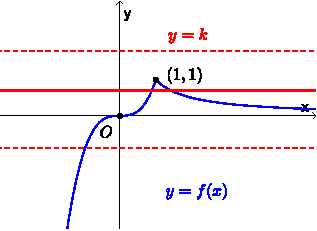
\includegraphics[scale=1]{2020-1217-1900-crop}
    \end{center}
\end{solution}



\section{2020 年 12 月 12 日答疑记录}

\subsection{弧度制}

角的大小用来描述角的两边 (始边和终边) 张开的幅度. 度量角的大小的方法中, 常见的为如下两种:

(1) 将射线绕定点旋转一周所形成的角 (称为周角) 等分为 $360$~份, 每一份的大小记为 $1^\circ$. 所以周角的大小是 $360^\circ$, 并这种方法称为角度制. 

(2) 将角的顶点放在圆心, 利用所截弧长来定义角的大小. 当圆心角固定时, 若半径越大, 则所对弧长也越大, 所以定义弧长与半径的比例为圆心角的大小, 并称这种方法为弧度制. 此时周角的大小是 $\dfrac{2\pi r}r= 2\pi\,\mathrm{rad}$. $\mathrm{rad}$ 是弧度制的单位, 念作 ``弧度'' (radian), 通常略去不写.

根据相似形对应线段或弧成比例, 对固定的圆心角, 弧长与半径的比例为定值, 所以第二种方法是合理的. 

    \begin{center}
        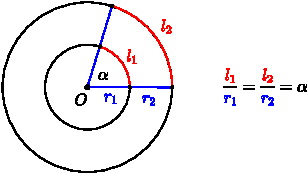
\includegraphics[scale=1]{2020-1218-1940-crop}
    \end{center}
    
高中数学更常用的是弧度制. 由定义, $360^\circ =2\pi$, 并应熟记特殊角 $0^\circ$, $30^\circ$, $45^\circ$, $60^\circ$, $90^\circ$, $120^\circ$, $135^\circ$, $150^\circ$, $180^\circ$ 的角度和弧度.

    \begin{center}
        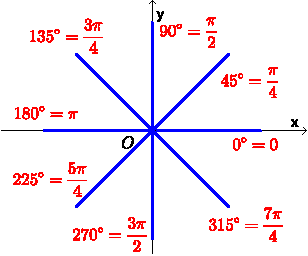
\includegraphics[scale=1]{2020-1220-0920-crop}\quad
        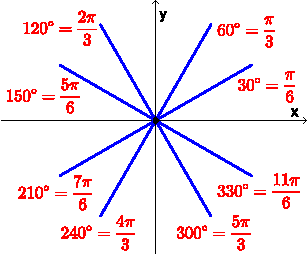
\includegraphics[scale=1]{2020-1220-0930-crop}
    \end{center}
    
容易得到弧度与角度互换公式: 
\[1\,\mathrm{rad}= \Big(\frac{180}{\pi}\Big)^{\circ} \approx 57.3^{\circ}, \quad
    1^{\circ}= \frac{\pi}{180}\,\mathrm{rad}.\]
若圆心角 $\alpha$ (弧度制, 可能为负) 所对的弧长为 $l$, 则 $|\alpha|=\dfrac{l}{r}$, 其中 $r$ 是圆的半径. 此外还有弧长公式 $l=|\alpha|r$, 和扇形面积公式
\[S= \dfrac{1}{2}lr= \dfrac{1}{2}|\alpha| r^2\quad 
    \text{(类似于三角形面积公式)}.\]

\begin{example}
    求终边落在直线 $y=-x$ 上的角 $\alpha$ 的集合.
\end{example}
\begin{solution}
    直线 $y=-x$ 为第二、四象限的角平分线, 作图易知, 所求集合为
    \[\{\alpha\mid\ 135^\circ+k\cdot 180^\circ\}
        = \biggl\{\alpha\biggm| \frac{3\pi}4+k\pi\biggr\}.\]
    以上两个集合, 只写其中一个即可 (用弧度制相对来说更简洁).
\end{solution}

\begin{example}\label{exa:201220-1030}
    已知某扇形的半径为 $10$, 面积为 $\dfrac{50\pi}3$, 求该扇形的圆心角大小.
\end{example}
\begin{solution}
    设该扇形的圆心角弧度大小为 $\alpha$, 半径为 $r$, 则其面积 \[S=\frac12\alpha r^2,\quad\text{即}\quad 
        \frac{50\pi}3= \frac12 \alpha\cdot 10^2.\]
    解得 $\alpha=\dfrac\pi3$.
\end{solution}
\begin{remark}
    例~\ref{exa:201220-1030} 也可以用角度制来解: 设该扇形的圆心角角度大小为 $\alpha$, 半径为 $r$, 则其面积 $S=\dfrac{\alpha}{360^\circ} \pi r^2$, 可求得 $\alpha=60^\circ$. 用角度制计算相对更简单一些.
\end{remark}

\subsection{任意角三角函数的定义}

  如下方左图, 设 $\alpha$ 是任意一个角, 顶点为坐标原点, 
  始边为 $x$~正半轴, $P(x, y)$ 是终边上任意一点 (异于原点), 
  它与原点的距离是 $r= \sqrt{x^2+ y^2}> 0$, 那么 
  \[\sin\alpha= \frac{y}{r},\quad
    \cos\alpha= \frac{x}{r},\quad 
    \tan\alpha= \frac{y}{x}\ (x\neq 0).\]
  三角函数值只与角的大小有关, 而与终边上点~$P$ 的位置无关. 由定义容易判断各象限内的角的三角函数值的正负号. 若点~$P$ 恰在单位圆 (圆心为原点且半径为 $1$) 上, 取点~$A(1,0)$, 并作 $PM\perp OA$ 于点 $M$, 作 $TA\perp OA$ 并交射线~$OP$ 于点~$T$, 则此时 $r=1$, 且 (类似锐角三角函数的定义)
  \[\sin\alpha= y,\quad
    \cos\alpha= x,\quad 
    \tan\alpha= \frac{AT}{OA}= AT\ (x\neq 0).\]
  对 $\angle{POA}$ 来说, $MP$ 为正弦线, $OM$ 为余弦线, $AT$ 为正切线, 
  且各线段均为有向线段 (即规定了正方向, 所以表示时带正负号). 常用的三角函数值, 参考下方右图. 由此可以写出其他特殊角 ($120^\circ$, $135^\circ$, $150^\circ$ 等) 的各三角函数值, 如 $\sin 120^\circ= \dfrac{\sqrt3}2$, $\cos135^\circ= -\dfrac{\sqrt2}2$.
  
  \begin{small}
    \begin{minipage}[t]{0.35\linewidth}
    \centering
    \begin{tikzpicture}[scale=1.1]
      \draw[-{Stealth[scale=0.8]}] (-1.2,0) -- (1.4,0) node[below] {$x$};
      \draw[-{Stealth[scale=0.8]}] (0,-1.2) -- (0,1.3) node[left] {$y$};
      \draw (0,0) circle (1) node[anchor=45] {$O$} coordinate (O);
      \def\myangle{40};
      \pgfmathparse{tan(\myangle)};
      \coordinate (B) at (\myangle:1.6);
      \draw[fill=black] (1,0) circle (0.6pt) coordinate (A)
        +(0.1,0) node[below] {$A$};
      \draw[fill=black] (1,\pgfmathresult) coordinate (T) circle (0.6pt) 
        node[above] {$T$} ;
      \draw[fill=black] (\myangle:1) circle (0.6pt) coordinate (P)
       +(0,0.06) node[above] {$P$};
      \draw[fill=black] ($(O)!(P)!(A)$) coordinate (M) circle (0.6pt) 
        node[below] {$M$};
      \draw (O)--(B) (M)--(P) (A)--(T);      
    \end{tikzpicture}
    \end{minipage}
    \hskip 1cm%
    \begin{minipage}[t]{0.55\linewidth}
    \centering
    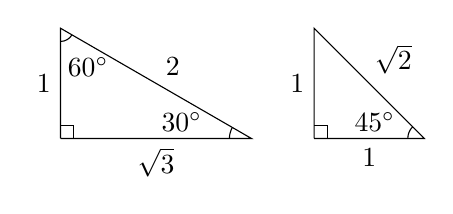
\begin{tikzpicture}[scale=1.4]
      \pgfmathparse{sqrt(3)};
      \draw (0,0) coordinate (A)-- node[below] {$\sqrt3$} 
        (1.732,0) coordinate (B)-- node[anchor=225] {$2$}
        (0,1) coordinate (C)--node[left] {$1$} (0,0);
      \draw (A)++(0,0.12)--++(0.12,0)--++(0,-0.12);
      \draw (C)+(0,-0.12) arc (270:330:0.12);
      \draw (B)+(-0.2,0) arc (180:150:0.2);
      \draw (A)+(0.25,0.65) node {$60^\circ$} +(1.1,0.15) node {$30^\circ$};
      \draw (2.3,0) coordinate (D)-- node[below] {$1$} 
        +(1,0) coordinate (E)-- node[anchor=225] {$\sqrt2$}
        +(0,1) coordinate (F)--node[left] {$1$} (2.3,0);
      \draw (D)++(0,0.12)--++(0.12,0)--++(0,-0.12);
      \draw (E)+(-0.15,0) arc (180:135:0.15);
      \draw (D)+(0.55,0.15) node {$45^\circ$};
    \end{tikzpicture}
    \end{minipage}
    \end{small}

\begin{example}
    $\sin6\underline{\qquad}0$. (填 ``$>$'' 或 ``$<$'')
\end{example}
\begin{solution}
    注意题中的 $6$ 是弧度制, 而 $360^\circ=2\pi\approx 6.28$, 所以 $6$~弧度在第四象限. 由正弦的定义, $\sin 6<0$.
\end{solution}
\begin{remark}
    类似地, $1$~弧度在第一象限, $2$ 弧度和 $3$ 弧度都在第二象限, 所以
    \[\sin 1,\ \sin 2,\ \sin 3>0,\quad 
        \cos 1>0,\quad \cos 2,\ \cos 3<0.\]
    此外, 画图可知 $\sin 1< \sin 2$.
\end{remark}

\begin{example}
    已知角 $\alpha$ 的终边经过点 $P(-x,-12)$, 
    且 $\cos\alpha=-\dfrac5{13}$, 求 $x$ 的值.
\end{example}
\begin{solution}
    由余弦定义, 
    \[\cos\alpha= \frac{-x}{\sqrt{(-x)^2+(-12)^2}}= -\frac5{13},\quad
    \text{解得}\ x=\pm5.\]
    经检验, $x=5$  (或由余弦值为负知点~$P$ 在第二、三象限, 所以 $-x<0$ 即 $x>0$).
\end{solution}
\section{2020 年 12 月 13 日答疑记录}

\begin{example}
    求函数 $f(x)=4^x-2^x-2$ 的零点.
\end{example}
\begin{solution}
    令 $f(x)=0$, 则 $4^x-2^x-2=0$, 即
    \[(2^x)^2-2^x-2=0,\quad (2^x-2)(2^x+1)=0.\]
    因为恒有 $2^x>0$, 所以 $2^x=2$, 解得 $x=1$. 故所求零点为 $x=1$. 
\end{solution}

\begin{example}\label{exa:201223-1850}
    设方程 $2^{-x}= |\lg x|$ 的两个根为 $x_1$, $x_2$, 求 $x_1x_2$ 的取值范围.
\end{example}
\begin{solution}
    分别画出函数 $f(x)= 2^{-x}$ 和 $g(x)= |\lg x|$ 的图形, 可知两者交点的横坐标为 $x_1$, $x_2$, 且均为正数并分别在 $1$ 的两侧. 不妨设 $x_1\in(0,1)$, $x_2\in(1,+\infty)$, 由 $f(x)$ 单调递减可知, $f(x_1)>f(x_2)$, 即 $g(x_1)>g(x_2)$, 所以
    \[|\lg x_1|> |\lg x_2|,\quad -\lg x_1> \lg x_2,\]
    整理可得 $\lg (x_1x_2)<0$. 进一步有 $x_1x_2\in(0,1)$.
    
    \begin{center}
        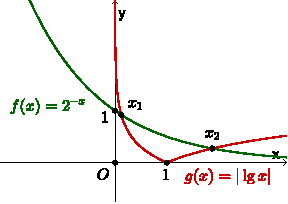
\includegraphics[scale=1]{2020-1223-1900-crop}
    \end{center}
\end{solution}
\begin{remark}
    若将例~\ref{exa:201223-1850} 中的方程改为 $k= |\log_a x|$, 其中 $k$ 为正的常数, $a\in(0,1)\cup (1,+\infty)$, 用同样的方法可以知道 $x_1x_2=1$.
\end{remark}

\begin{example}
    一个容器装有细沙 $a\,\text{cm}^3$, 细沙从容器底部一个细微的小孔慢慢地匀速漏出, $t\,\text{min}$ 后剩余的细沙量为 $y= a\mathrm{e}^{-bt}\,(\text{cm}^3)$, 经过 $8\,\text{min}$ 后发现容器内还有一半的沙子, 求需要再经过多少时间, 容器中的沙子只有开始时的八分之一.
\end{example}
\begin{solution}
    设经过 $t\,\text{min}$ 符合题意, 则由已知,
    \[\left\{\!\!\begin{array}{l}
        a\mathrm{e}^{-b\cdot 8}= \dfrac{a}2,\\[5pt]
        a\mathrm{e}^{-bt}= \dfrac{a}8,
        \end{array}\right.\ \text{即}
      \left\{\!\!\begin{array}{l}
        \mathrm{e}^{-8b}= \dfrac12,\\[3pt]
        \mathrm{e}^{-bt}= \dfrac18.
      \end{array}\right.\]
    因为 $\dfrac18= \biggl(\dfrac12\biggr)^3$, 所以
    \[\mathrm{e}^{-bt}= (\mathrm{e}^{-8b})^3= \mathrm{e}^{-24b},\]
    即 $-bt=-24b$, 解得 $t=24$. 这表明需要再经过 $(t-8)\,\text{min}= 16\,\text{min}$, 才能符合题意.
\end{solution}

\begin{example}
    设函数 $f(x)= \log_{\frac12} x$, 求下列命题中真命题的个数:
    
    (1) 函数 $f(|x|)$ 为偶函数.
    
    (2) 若 $f(a)= |f(b)|$, 其中 $a$, $b>0$ 且 $a\neq b$, 则 $ab=1$.
    
    (3) 函数 $f(-x^2+2x)$ 在 $(1,3)$ 上为单调递增函数.
    
    (4) 若 $0<a<1$, 则 $|f(1+a)|< |f(1-a)|$.   
\end{example}
\begin{solution}
    (1) 设 $g(x)=f(|x|)$, 则 
    \[g(-x)= f(|-x|)= f(|x|)= g(x),\]
    所以函数 $f(|x|)$ 为偶函数 (此结论无需考虑 $f(x)$ 的具体表达式).
    
    (2) $f(x)= |f(b)|$ 化为 $\log_{\frac12} a= |\log_{\frac12} b|$, 由此可知 $\log_{\frac12} a\geqslant 0$, 即 $a\in(0,1]$. 若 $b\in(0,1]$, 则 $\log_{\frac12} a= \log_{\frac12} b$, 必有 $a=b$, 与已知矛盾. 若 $b\in(1,+\infty)$, 则 
    \[\log_{\frac12} a= -\log_{\frac12} b,\quad\text{即}\quad
        \log_{\frac12} ab=0,\]
    所以 $ab=1$.
    
    (3) 函数 $f(-x^2+2x)= \log_{\frac12}(-x^2+2x)$, 定义域为 $(0,2)$, 所以在 $(1,3)$ 并非处处有定义, 无法判断定义域. (如果只考虑 $x\in(1,2)$, 则可由复合函数的单调性知, 函数 $f(-x^2+2x)$ 为单调递增函数.)
    
    (4) 方法一: 因为 $0<a<1$, 所以 $1-a\in(0,1)$, $1+a\in(1,2)$,
    \[\begin{aligned}
        |f(1+a)|- |f(1-a)|
        &= |\log_{\frac12} (1+a)|- |\log_{\frac12} (1-a)|\\
        &= -\log_{\frac12} (1+a)- \log_{\frac12} (1-a)\\
        &= -\log_{\frac12} (1-a^2)<0,
    \end{aligned}\] 
    即 $|f(1+a)|- |f(1-a)|<0$, 因此 $|f(1+a)|< |f(1-a)|$.
    
    方法二: 直接画函数 $h(x)= |\log_{\frac12} x|$ 的图形, 并由图形单调性可知,
    \[|f(1+a)|< |f(1-a)|.\]
    
    \begin{center}
        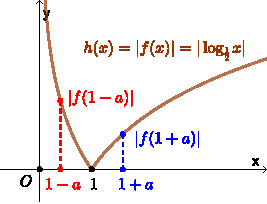
\includegraphics[scale=1]{2020-1223-1940-crop}
    \end{center}
    
    综上所述, (1)(2)(4) 是真命题, 共 $3$ 个.
\end{solution}

\begin{example}
    已知函数 $f(x)= \dfrac{2x+1}{x+1}$, 求该函数在区间 $[1,4]$ 上的最大值与最小值.
\end{example}
\begin{solution}
    用分离常数法, 
    \[f(x)= \frac{2x+1}{x+1}= \frac{2(x+1)-1}{x+1}
        = 2-\frac1{x+1}.\]
    因为 $x\in[1,4]$, 所以 $\dfrac1{x+1}$ 单调递减, $-\dfrac1{x+1}$ 单调递增, $2-\dfrac1{x+1}$ 也单调递增, 从而 
    \[f_{\min}= f(1)= \dfrac32,\quad f_{\max}= f(4)= \dfrac95.\]
\end{solution}

\begin{example}
    大气中的温度随着高度的上升而降低, 根据实测的结果, 上升到 $12\,\text{km}$ 为止温度的降低大体上与升高的距离成正比, 在 $12\,\text{km}$ 以上温度一定, 保持在 $-55\,\textcelsius$.
    
    (1) 当地表大气的温度是 $a\,\textcelsius$ 时, 在 $x\,\text{km}$ 上空的温度为 $y\,\textcelsius$, 求 $a$, $x$, $y$ 之间的函数关系式;
    
    (2) 当地表大气的温度是 $29\,\textcelsius$ 时, 在 $3\,\text{km}$ 上空的温度是多少?
\end{example}
\begin{solution}
    (1) 设题中的正比例系数为 $k$, 则 $a-y=kx$. 因为当 $x=12$ 时, $y=-55$, 所以 
    \[a-(-55)= k\cdot 12,\quad\text{即}\quad
        k= \frac{a+55}{12}.\]
    进一步可得,
    \[y=\begin{cases}
        a-\dfrac{a+55}{12}, & x\in[0,12],\\
        -55, & x\in(12,+\infty).
    \end{cases}\]
    
    (2) 此时 $a=29$, 当 $x=3$ 时, $y=29 -\dfrac{29+55}{12}=22$.
\end{solution}

\begin{example}
    已知函数 $f(x)= \log_a (2-x)+\log_a(x+2)$ 的最小值为 $-4$, 其中 $0<a<1$, 求 $a$ 的值.
\end{example}
\begin{solution}
    由题意,
    \[\left\{\!\!\begin{array}{l}
        2-x>0,\\
        x+2>0,
      \end{array}\right.\ \text{解得}\quad x\in(-2,2).\]
    因为 $f(x)= \log_a (4-x^2)$, 而 $4-x^2\in(0,4]$, 所以由 $\log_a x$ 单调递减可知, $f(x)\in[\log_a 4,+\infty)$. 因此 
    \[\log_a 4=-4,\quad a^{-4}= 4,\quad
        a= 4^{-\frac14}= \frac{\sqrt2}2.\]
\end{solution}

\begin{example}
    已知 $\log_a \dfrac23<1$, 求实数 $a$ 的取值范围.
\end{example}
\begin{solution}
    不等式化为 $\log_a \dfrac23< \log_a a$.

    (1) 若 $a\in(0,1)$, 由 $\log_a x$ 单调递减可知, $a<\dfrac23$, 所以 $a\in\biggl(0,\dfrac23\biggr)$.
    
    (2) 若 $a\in(1,+\infty)$, 由 $\log_a x$ 单调递增可知, $a>\dfrac23$, 所以 $a\in(1,+\infty)$.
    
    综上所述, $a\in\biggl(0,\dfrac23\biggr)\cup(1,+\infty)$.
\end{solution}

\begin{example}
    若函数 $y= 2^{|x-1|}$ 在区间 $(k-1,k+1)$ 内不单调, 求 $k$ 的取值范围.
\end{example}
\begin{solution}
    由 $y=2^|x|$ 的图形向右平移一个单位长度可得 $y= 2^{|x-1|}$ 的图形, 而前者为偶函数, 且当 $x\geqslant 0$ 时 $y=2^x$. 由此可以画出 $y= 2^{|x-1|}$ 的图形如下:
    
    \begin{center}
        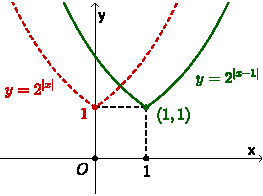
\includegraphics[scale=1]{2020-1223-2000-crop}
    \end{center}
    
    由图可知, $y= 2^{|x-1|}$ 在 $(-\infty,1)$ 上单调递减, 在 $(1,+\infty)$ 上单调递增. 因为题中要求函数 $y= 2^{|x-1|}$ 在区间 $(k-1,k+1)$ 内不单调, 所以
    \[1\in(k-1,k+1),\quad\text{解得}\quad k\in(0,2).\]
\end{solution}
\section{2020 年 12 月 16 日答疑记录}

    同角三角函数有两个常用基本关系式: 
  \[\sin^2 x+ \cos^2 x= 1,\quad 
    \tan x= \frac{\sin x}{\cos x}.\]
  后一个式子也可以认为是正切的定义. 前一个式子等价于勾股定理, 由该式可知
  \[\begin{gathered}
    (\sin x\pm \cos x)^2= 1\pm 2\sin x\cos x,\\
        \sin^2 x= 1-\cos^2 x= (1+\cos x)(1-\cos x).
  \end{gathered}\] 
  
\begin{example}
    已知 $\cos\alpha= -\dfrac35$, 且 $\tan\alpha>0$, 求 $\dfrac{\sin\alpha\cos^2\alpha}{1-\sin\alpha}$.
\end{example}
\begin{solution}
    方法一: 由题意, $\alpha$ 在第三象限, 所以 $\sin\alpha= -\dfrac45$, 
    \[\frac{\sin\alpha\cos^2\alpha}{1-\sin\alpha}
        = \frac{-\dfrac45\cdot\bigg(-\dfrac35\biggr)^2}{1- \biggl(-\dfrac45\biggr)}
        = -\frac{4}{25}.\]
    
    方法二: 也可以利用 $\cos^2\alpha= 1-\sin^2\alpha=(1+\sin\alpha)(1-\sin\alpha)$ 得,
    \[\frac{\sin\alpha\cos^2\alpha}{1-\sin\alpha}
        =\frac{\sin\alpha(1-\sin^2\alpha)}{1-\sin\alpha}
        = \sin\alpha(1+\sin\alpha)
        = -\frac{4}{25}.\]
\end{solution}

\begin{example}
    化简 $\dfrac{\cos\theta}{1+\cos\theta}- \dfrac{\cos\theta}{1-\cos\theta}$.
\end{example}
\begin{solution}
    通分后合并可知,
    \[\begin{aligned}
        \frac{\cos\theta}{1+\cos\theta}- \frac{\cos\theta}{1-\cos\theta}
        &= \frac{\cos\theta(1- \cos\theta- (1+ \cos\theta))}{(1- \cos\theta)(1+ \cos\theta)}\\
        &= \frac{\cos\theta(-2\cos\theta)}{1- \cos^2\theta}
         = -\frac{2\cos^2\theta}{\sin^2\theta}\\
        &= - \frac2{\tan^2\theta}.
    \end{aligned}\]
    其中最后一个等号及其后的式子可以不写.
\end{solution}

  凡正余弦的二次式, 均可以化成正切函数来表示, 例如:
  \[\sin x\cos x+ \cos^2 x
    = \frac{\sin x\cos x+ \cos^2 x}{\sin^2 x+ \cos^2 x}
    = \frac{\tan x+ 1}{\tan^2 x+ 1}.\]
  与此类似的还有
  \[\frac{\sin x+\cos x}{\sin x-\cos x}
    = \frac{\tan x+1}{\tan x-1}.\]
  这两种变形方法常用来解决正余弦值和正切值的转化问题.
  
\begin{example}
    已知 $\dfrac{\sin\theta+ \cos\theta}{\sin\theta- 2\cos\theta}= \dfrac12$, 求 $\tan\theta$.
\end{example}
\begin{solution}
    方法一: 原式分子、分母同除以 $\cos\theta$, 得 $\dfrac{\tan\theta+ 1}{\tan\theta- 2}= \dfrac12$, 所以 $\tan\theta= -4$.
    
    方法二: 将原式化为整式, 
    \[2(\sin\theta+ \cos\theta)=\sin\theta- 2\cos\theta,\]
    所以 $\sin\theta= -4\cos\theta$, 即 $\tan\theta= -4$.
\end{solution}

\begin{example}
    设角~$\alpha$ 的终边过点~$P(3,4)$, 求 $\dfrac{\sin\alpha+ 2\cos\alpha}{\sin\alpha- \cos\alpha}$.
\end{example}
\begin{solution}
    方法一: 由题意, $\tan\alpha= \dfrac43$, 所以
    \[\frac{\sin\alpha+ 2\cos\alpha}{\sin\alpha- \cos\alpha}
        = \frac{\tan\alpha+ 2}{\tan\alpha- 1}
        = 10.\]
    
    方法二: 由题意, $\dfrac{\sin\alpha}{\cos\alpha}= \dfrac43$, 即 $\sin\alpha= \dfrac43\cos\alpha$, 所以
    \[\frac{\sin\alpha+ 2\cos\alpha}{\sin\alpha- \cos\alpha}
        = \frac{\dfrac43\cos\alpha+ 2\cos\alpha}{\dfrac43\cos\alpha- \cos\alpha}
        = 10.\]
\end{solution}
\section{2020 年 12 月 18 日答疑记录}

  诱导公式指的是已知角加上 $90^\circ$ (或 $\dfrac{\pi}2$) 的整数倍后,
  所得角与已知角的三角函数值的关系. 最容易理解的是
  \[\sin(2\pi+\alpha)= \sin\alpha,\quad
        \cos(2\pi+\alpha)= \cos\alpha.\]
  常用的还有
  \[\begin{gathered}
    \sin(-x)= -\sin x\ (\text{奇函数}),\quad 
        \cos(-x)= \cos x\ (\text{偶函数}),\\
    \sin(90^\circ-x)= \cos x,\quad \cos(90^\circ-x)= \sin x,\\
    \sin(180^\circ-x)= \sin x,\quad \cos(180^\circ-x)= -\cos x.
  \end{gathered}\]
  分别对应如下图形 (为观察方便, 正弦线、余弦线的位置与通常的定义略有区别):
    \begin{center}
        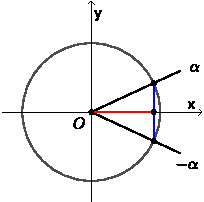
\includegraphics[scale=1.1]{2020-1225-1900-crop}\quad
        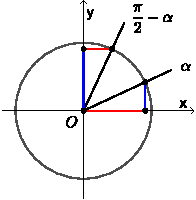
\includegraphics[scale=1.1]{2020-1225-1910-crop}\quad
        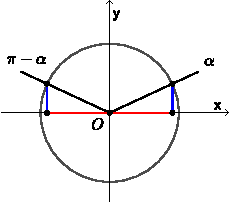
\includegraphics[scale=1.1]{2020-1225-1920-crop}
    \end{center}
  
  诱导公式的记忆口诀为: 奇变偶不变, 符号看象限, 其中
  
  (1) “奇”“偶”指所加 $90^\circ$ (或 $\dfrac{\pi}2$) 倍数的奇偶性; 
  
  (2) “变”指函数名中“正”变“余”或“余”变“正”;
  
  (3) “象限”指把已知角视为锐角时所得角对应的象限;
   
  (4) “符号”是此时原式的符号. \\
  例如:
  \begin{gather*}
    \sin(2x-\pi)= -\sin2x,\quad \tan(x+180^\circ)= \tan x, \\
    \cos(3x-270^\circ)= -\sin 3x,\quad
    \sin\Big(4x-\frac{\pi}2\Big)= -\cos 4x.
  \end{gather*}
    可结合如下图形理解诱导公式:
    \begin{center}
        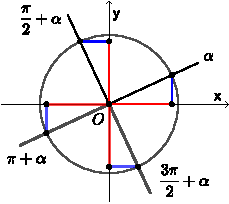
\includegraphics[scale=1.1]{2020-1225-1930-crop}
    \end{center}
    
    由上图可知:
    \[\begin{gathered}
        \sin\biggl(\frac\pi2+\alpha\biggr)= \cos\alpha,\quad
            \cos\biggl(\frac\pi2+\alpha\biggr)= -\sin\alpha,\\
        \sin(\pi+\alpha)= -\sin\alpha,\quad
            \cos(\pi+\alpha)= -\cos\alpha,\\
        \sin\biggl(\frac{3\pi}2+\alpha\biggr)= -\cos\alpha,\quad
            \cos\biggl(\frac{3\pi}2+\alpha\biggr)= \sin\alpha,
    \end{gathered}\]
    恰好验证了诱导公式.
    
\begin{example}
    化简: $\dfrac{\sin\biggl(\alpha-\dfrac{11}2\pi\biggr)
        \cos\biggl(\dfrac{\pi}2-\alpha\biggr)
        \tan(2\pi-\alpha)}{\cos\biggl(\dfrac{\pi}2+\alpha\biggr)
        \cos(\alpha-2\pi)\tan(\alpha-5\pi)}$.
\end{example}
\begin{solution}
    由诱导公式,
    \[\begin{gathered}
        \sin\biggl(\alpha-\dfrac{11}2\pi\biggr)
        = \sin\biggl(\alpha-\dfrac{3}2\pi\biggr)
        = \sin\biggl(\alpha+\dfrac{\pi}2\biggr)
        = \cos\alpha,\\
        \cos\biggl(\dfrac{\pi}2-\alpha\biggr)= \sin\alpha,\qquad
        \tan(2\pi-\alpha)= \tan(-\alpha)= -\tan\alpha,\\
        \cos\biggl(\dfrac{\pi}2+\alpha\biggr)= -\sin\alpha,\qquad
        \cos(\alpha-2\pi)= \cos\alpha,\\
        \tan(\alpha-5\pi)= \tan(\alpha+\pi)= \tan\alpha,
    \end{gathered}\]
    所以
    \[\text{原式}= \frac{\cos\alpha\sin\alpha(-\tan\alpha)}{
        -\sin\alpha\cos\alpha\tan\alpha}= 1.\]
\end{solution}

    用诱导公式解题时, 应先利用本节第一个公式, 将式中 $\pi$ 的系数的绝对值尽可能变小, 最好是将含 $\pi$ 的项化为 $[-\pi,\pi]$ 内的数.



\section{2020 年 12 月 22 日答疑记录}

本次答疑记录是 12 月数学月考里选择、填空题的错题讲解, 原先为两次答疑的内容. 为了方便起见, 所有题均改成解答题, 并整合成一次记录. 

\begin{example}
    已知函数 $f(x)=2-\dfrac3x$, 若 $g(x)= f(x)-m$ 为奇函数, 求实数 $m$ 的值.
\end{example}
\begin{solution}
    方法一: 由题意, $g(x)=2-\dfrac3x-m$ 且 $g(-x)= -g(x)$, 所以
    \[2-\dfrac3{-x}-m= -\biggl(2-\dfrac3x-m\biggl),\quad
        \text{整理得}\quad m=2.\]
    
    方法二: 因为 $f(x)=2-\dfrac3x$ 的图形可由 $y=-\dfrac3x$ 的图形向上平移两个单位长度得到, 而后者关于原点对称 (函数为奇函数), 而 $g(x)= f(x)-m$ 的图形可由 $f(x)$ 的图形上、下平移得到, 所以只需 $m=2$, 即将 $f(x)$ 的图形向下平移两个单位长度, 可得 $g(x)=-\dfrac3x$ 为奇函数.
\end{solution}

\begin{example}
    ``$\ln a>\ln b$'' 是 ``$3^a>3^b$'' 的什么条件?
\end{example}
\begin{solution}
    有 $y=\ln x$ 的定义域为 $(0,+\infty)$ 且单调递增, 可知 $\ln a>\ln b$ 表明 $a>b>0$. 再由 $y=3^x$ 的定义域为 $\realnum$ 且单调递增, 可知 $3^a>3^b$ 表明 $a>b$. 因此 ``$\ln a>\ln b$'' 是 ``$3^a>3^b$'' 的必要不充分条件.
\end{solution}


\begin{example}
    根据有关资料, 围棋状态空间复杂度的上限 $M$ 约为 $3^{361}$, 而可观测宇宙中普通物质的原子总数 $N$ 约为 $10^{80}$. 将 $\dfrac{M}{N}$ 表示为 $10$ 的正整数次方 ($\lg 3\approx 0.48$).
\end{example}
\begin{solution}
    根据对数的运算性质, 
    \[\begin{aligned}
        \lg \dfrac{M}{N}
        &= \lg M-\lg N= \lg 3^{361}- \lg 10^{80}
         = 361\lg 3- 80\\
        &\approx 361\cdot 0.48- 80
         = 93.28,
       \end{aligned}\]
    所以 $\dfrac{M}{N}\approx 10^{93}$.
\end{solution}

\begin{example}
    画出函数 $y= \dfrac{x a^x}{|x|}$ ($0<a<1$) 的图形的大致形状.
\end{example}
\begin{solution}
    利用绝对值的定义, 原函数化为 $y= \begin{cases}
        -a^x, & x<0,\\
        a^x, & x>0,
    \end{cases}$
    图形的大致形状如下:
    
    \begin{center}
        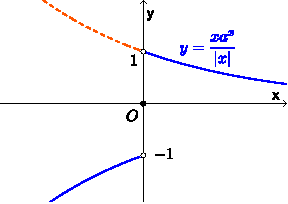
\includegraphics[scale=1.1]{2020-1227-1100-crop}
    \end{center}
\end{solution}


\begin{example}\label{exa:201227-1450}
    求关于 $x$ 的方程 $x=\log_a (-x^2 +2x+a)$ ($a>0$, 且 $a\neq 1$) 的解的个数.
\end{example}
\begin{solution}
    因为 $x=\log_a a^x$, 所以原方程化为
    \[\log_a a^x=\log_a (-x^2 +2x+a),\quad\text{即}\quad
        a^x= -(x-1)^2 +1+a,\]
    故应考虑函数 $f(x)=a^x$ 与 $g(x)= -(x-1)^2 +1+a$ 的图形的交点个数. 分 $0<a<1$ 和 $a>1$ 两种情况画图如下:
    
    \begin{center}
        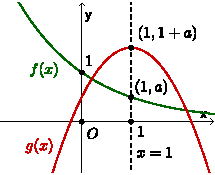
\includegraphics[scale=1.1]{2020-1227-1200-crop}\qquad
        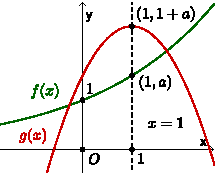
\includegraphics[scale=1.1]{2020-1227-1210-crop}
    \end{center}
    
    由图可知, $f(x)=a^x$ 与 $g(x)= -(x-1)^2 +1+a$ 的图形总有两个交点, 所以方程 $x=\log_a (-x^2 +2x+a)$ 的解的个数为 $2$.
\end{solution}

例~\ref{exa:201227-1450} 也可以直接画原方程 $x=\log_a (-x^2 +2x+a)$ 对应的两个函数 $y=x$ 和 $y=\log_a (-x^2 +2x+a)$ 的大致图形, 画后者之前需适当讨论, 略微麻烦一点.

\begin{example}
    若 $a>b$, 则下列不等式中哪些一定成立?
    
    (1) $\log_2 a> \log_2 b$;\quad 
    (2) $2^a> 2^b$;\quad 
    (3) $a^{\frac13}> b^{\frac13}$;\quad
    (4) $\dfrac1a<\dfrac1b$.
\end{example}
\begin{solution}
    此题主要考查函数的定义域和单调性.
    
    (1) 因为函数 $y=\log_2 x$ 的定义域为 $(0,+\infty)$ 且单调递增, 所以 $\log_2 a> \log_2 b$ 等价于 $a>b>0$, 与已知条件 $a>b$ 不符.
    
    (2) 因为函数 $y= 2^x$ 的定义域为 $\realnum$ 且单调递增, 所以 $2^a> 2^b$ 等价于 $a>b$, 与已知条件 $a>b$ 相同.
    
    (3) 因为函数 $y= x^{\frac13}$ 的定义域为 $\realnum$ 且单调递增, 所以 $a^{\frac13}> b^{\frac13}$ 等价于 $a>b$, 与已知条件 $a>b$ 相同.
    
    (4) 函数 $y=\dfrac1x$ 的定义域为 $(-\infty,0)\cup(0,+\infty)$, 所以 $\dfrac1a<\dfrac1b$ 不一定有意义 (如当 $a=0$ 或 $b=0$ 时). 即使该式有意义, 在已知条件 $a>b$ 中取 $a>0$, $b<0$ 可知 $\dfrac1a>0>\dfrac1b$, 与本小题结论不符.
\end{solution}


\begin{example}
    下列各式中哪些是正确的?
    
    (1) $\sin\dfrac\pi5> \sin\dfrac{6\pi}5$;\quad 
    (2) $\cos\biggl(-\dfrac\pi3\biggr)< \cos\dfrac\pi6$;
    
    (3) $\tan\dfrac\pi4> \tan\dfrac{5\pi}4$;\quad 
    (4) $\sin\dfrac\pi3> \sin\dfrac\pi6$.
\end{example}
\begin{solution}
    画正弦线、余弦线如下:
    
    \begin{center}
        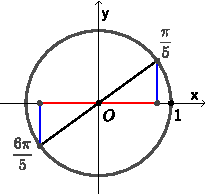
\includegraphics[scale=1.1]{2020-1227-1300-crop}\qquad
        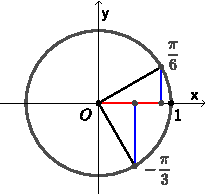
\includegraphics[scale=1.1]{2020-1227-1310-crop}\\[5pt]
        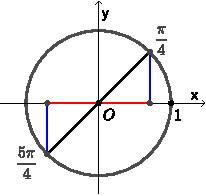
\includegraphics[scale=1.1]{2020-1227-1320-crop}\qquad
        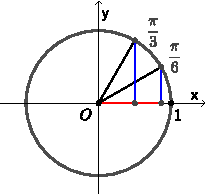
\includegraphics[scale=1.1]{2020-1227-1330-crop}
    \end{center}
    
    由此可知 (正切值由正弦值比余弦值得到)
    \[\begin{gathered}
        \sin\dfrac\pi5>0> \sin\dfrac{6\pi}5,\quad 
        \cos\biggl(-\dfrac\pi3\biggr)=\frac12< \frac{\sqrt3}2=\cos\dfrac\pi6,\\
        \tan\dfrac\pi4= 1= \tan\dfrac{5\pi}4,\quad 
        \sin\dfrac\pi3= \frac{\sqrt{3}}2> \frac12=\sin\dfrac\pi6.
    \end{gathered}\]
\end{solution}

\begin{example}\label{exa:201227-1440}
    已知 $f(x)$ 是定义在 $\realnum$ 上的偶函数, 且当 $x\in(-\infty,0]$ 时, $f(x)=2^x+\dfrac13$, 求 $f\biggl(\log_2 \dfrac32\biggr)$ 的值.
\end{example}
\begin{solution}
    因为 $\log_2 \frac32>\log_2 1=0$, 所以由偶函数的特征,
    \[f\biggl(\log_2 \frac32\biggr)= f(-x)
        = 2^{-\log_2 \frac32}+\frac13
        = 2^{\log_2 \frac23}+\frac13
        = \frac23+\frac13= 1.\]
\end{solution}

例~\ref{exa:201227-1440} 中也可以先求 $f(x)$ 在 $x\in(0,+\infty)$ 时的解析式, 可参考 ``2020 年 11 月 14 日答疑记录'' 的第五个例子和 ``2020 年 11 月 22 日答疑记录'' 的第二个例子. 

\begin{example}
    已知函数 $f(x) =\begin{cases}
        3^x, & x\leqslant 0,\\
        -2x+1, & x>0,
    \end{cases}$ 若 $f(x)\leqslant \dfrac13$, 求实数 $x$ 的取值范围.
\end{example}
\begin{solution}
    (1) 若 $x\leqslant 0$, 则 $f(x)\leqslant \dfrac13$ 化为
    \[3^x\leqslant \frac13= 3^{-1},\quad\text{解得}\quad
        x\leqslant -1.\]
    
    (2) 若 $x> 0$, 则 $f(x)\leqslant \dfrac13$ 化为
    \[-2x+1\leqslant \frac13,\quad\text{解得}\quad
        x\geqslant \frac13.\]
        
    综上所述, $x\in (-\infty,-1]\cup \biggl[\dfrac13,+\infty\biggr)$.
\end{solution}

分段函数分段考虑, 下题也是如此.

\begin{example}
    已知函数 $f(x)= \begin{cases}
        ax+2-3a, & x<0,\\
        2^x-1, & x\geqslant 0.
    \end{cases}$ 若存在 $x_1$, $x_2\in\realnum$, $x_1\neq x_2$, 使得 $f(x_2)= f(x_2)$ 成立, 求实数 $a$ 的取值范围.
\end{example}
\begin{solution}
    题中 $f(x)$ 的图形在 $x<0$ 的部分为半直线, 在 $x\geqslant 0$ 的部分为 $y=2^x$ 向下平移一个单位长度. 而条件 ``存在 $x_1\neq x_2$ 使得 $f(x_2)= f(x_2)$ 成立'' 表明存在水平的直线与 $f(x)$ 的图形有两个不同的交点. 分 $a<0$, $a=0$ 和 $a>0$ 三种情况 (分别对应半直线不同的增减性) 画图如下:
    
    \begin{center}
        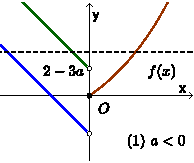
\includegraphics[scale=1.1]{2020-1227-1400-crop}\qquad
        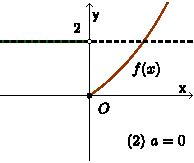
\includegraphics[scale=1.1]{2020-1227-1410-crop}\qquad
        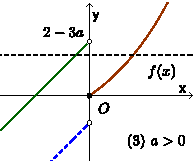
\includegraphics[scale=1.1]{2020-1227-1420-crop}
    \end{center}
    
    由图可知, 当 $a\leqslant 0$ 时, 图形均合题意; 而当 $a>0$ 时, 需 $2-3a>0$ 即 $a<\dfrac23$. 由此可知, 实数 $a$ 的取值范围为 $\biggl(-\infty,-\dfrac23\biggr)$.
\end{solution}
%\input{2020-1226}
%\input{2020-1229}



\end{document}

\begin{example}
    
\end{example}
\begin{solution}
    
\end{solution}

\begin{example}
    
\end{example}
\begin{solution}
    
\end{solution}


\left\{\!\!\begin{array}{l}
    ,\\
    
    \end{array}\right.

    \begin{center}
        \includegraphics[scale=1]{2020-1227-1900-crop}
    \end{center}